\section{Evaluation}
\label{sec:evaluation}

We now demonstrate performance improvements brought by our GPU
implementations for the existing vehicle detection program
\cite{Niknejad12}.
We also discuss the details of performance comparisons among our GPU
implementations and traditional CPU implementations identifying the
fundamental factors that allowed the GPU to outperform the CPU.

\subsection{Experimental Setup}
\label{sec:setup}

We prepare three variants of the vehicle detection program implemented
using (i) a single core of the multicore CPU, (ii) multiple cores of the
multicore CPU, (iii) and massively parallel compute cores of the GPU.
The CPU implementations use the Intel Core i7 3930K series while we
provide several varied GPUs for the GPU implementations: namely NVIDIA
GeForce GTX 560 Ti, GTX 580, GTX 680, TITAN, and K20Xm.
The same set of 10 images as previous work \cite{Niknejad12} is used as
input data and their average computation time is considered as a major
performance metrics.
Note that this computation time includes all relevant pieces of image
processing such as image loading and output rendering in addition to the
primary object detection part.

\subsection{Experimental Results}
\label{sec:results}

\begin{figure}[t]
 \begin{center}
  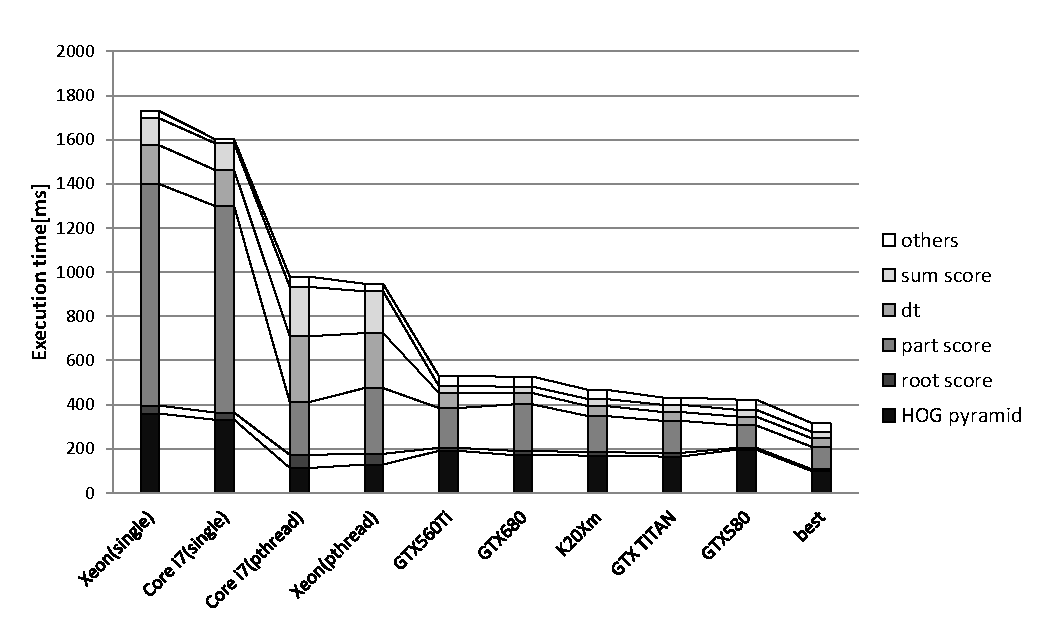
\includegraphics[width=\hsize]{fig/float_exe_time.eps}\\
  \caption{computation times of the single precision floating point program.}
  \label{fig:float_exe_time}
 \end{center}
\end{figure}

\begin{figure}[t]
 \begin{center}
  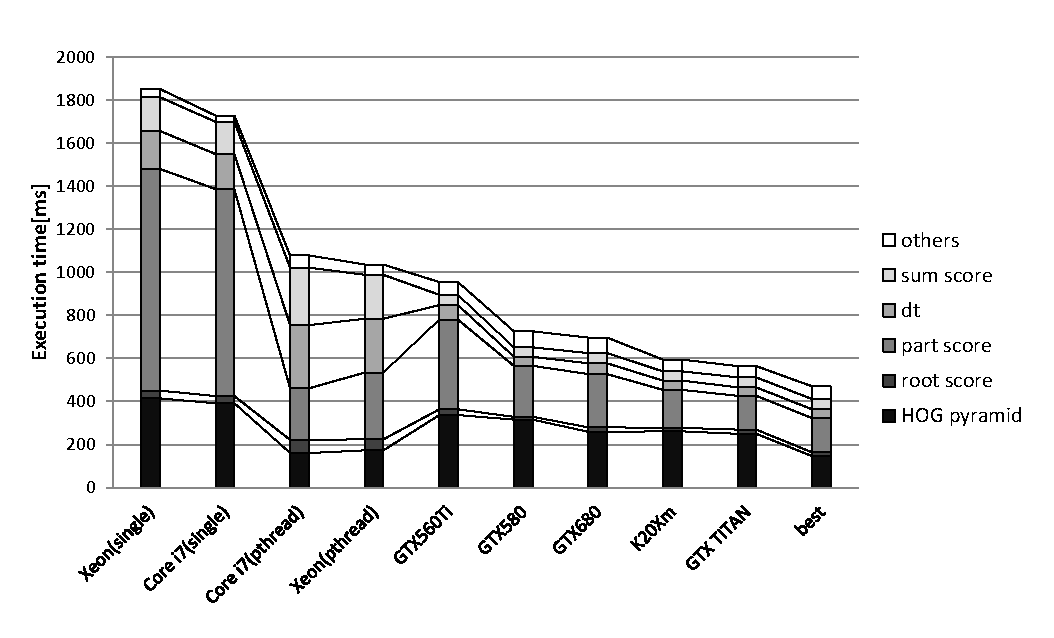
\includegraphics[width=\hsize]{fig/double_exe_time.eps}\\
  \caption{computation times of the double precision floating point program.}
  \label{fig:double_exe_time}
 \end{center}
\end{figure}

Fig.~\ref{fig:float_exe_time} shows the computation times of all variants
of the vehicle detection program configured to use the single precision
for floating operations.
The dimensions of input images are 640$\times$480 pixels.
``sequential'' uses a single CPU core while ``multicore'' uses multiple
CPU cores with \textit{pthread}.
Other labels except for ``best'' represent our GPU implementations using
corresponding GPUs.
``best'' is the best combination of the GPU and CPU implementations.
Most computational blocks benefit from GPUs; only the HOG calculation
prefers the multicore implementation.
This is attributed to the fact that the HOG calculation contains atomic
operations that squeeze massively parallel threads of the GPU.

A comparison of different GPUs provides an interesting observation.
The GPUs based on the state-of-the-art \textit{Kepler}
architecture \cite{NVIDIA_Kepler} are inferior to those based on the
previous \textit{Fermi} architecture \cite{NVIDIA_Fermi}.
The Kepler GPUs employ a significant number of compute cores with the
enhanced multithreading mechanism.
However they operate at a lower frequency than the Fermi GPUs due to
their complex architecture.
Since the vehicle detection program is compute-intensive as depicted
through Listing~\ref{lst:score} to \ref{lst:hog}, the operating 
frequency is more dominating than the architectural benefit.
This is a useful finding toward the future development of GPU-based
image processing.

As a result, the best performance is obtained from such a setup that
uses the multicore implementation for the HOG calculation while using
the GeForce GTX 580 GPU for other computational blocks offloaded.
It speeds up the execution of vehicle detection by more than 5x over the
traditional single-core CPU implementation and 3x over the multicore CPU
implementation respectively. 
A 3$\sim$5x speed-up for the overall execution of a complex real-world
application program is a significant contribution, whereas often an
order-of-magnitude speed-up is reported for a particular part of the
program or the algorithm.

Fig. \ref{fig:double_exe_time} shows the computation times of all variants
of the vehicle detection problem configuired to use the double precision
for floating operations.
Unlike the single-precision scenario, the Kepler GPUs outperform the
Fermi GPUs.
This explains that the double-precision performance of GPUs is improved
as the generation of GPUs advances.
Another notable finding is that the TITAN GPU is slightly faster than
the K20Xm GPU for our vehicle detection program.
This is due to a slightly higher operating frequency of the TITAN GPU.
Since the TITAN GPU is a consumer market price while the K20Xm is a very
expensive supercomputing device, we suggest that the vehicle detection
program uses the TITAN GPU for a better cost performance.

\begin{figure}[t]
 \begin{center}
  \includegraphics[width=\hsize]{fig/time_on_image_size.eps}\\
  \caption{Impact of the image size on computation times.}
  \label{fig:time_on_image_size}
 \end{center}
\end{figure}

Fig. \ref{fig:time_on_image_size} shows the impact of the image size on
computation times. 
We herein use the program configured to use the single precision for
floating-point operations.
The GPU implementation uses the GeForce GTX 580 GPU, which is the best
performer in all the GPUs demonstrated in Fig. \ref{fig:float_exe_time}.
The lessons learned from this experiment are that the execution time of
the vehicle detection program is proportionally influenced by the input
image size.
This means that the benefit of our GPU implementations as compared to
the traditional CPU implementations would hold for more high-resolution
image processing.

\begin{figure}[t]
 \begin{center}
  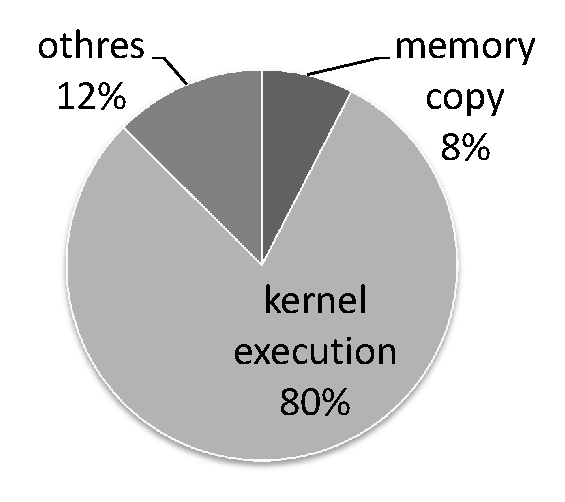
\includegraphics[width=0.6\hsize]{fig/breakdown_gpu.eps}\\
  \caption{The breakdown of computation times of the GPU implementation.}
  \label{fig:breakdown_gpu}
 \end{center}
\end{figure}

Fig. \ref{fig:breakdown_gpu} shows the breakdown of computation times of
the GPU implementation that achieves the best performance for the single
precision vehicle detection program.
The memory copy overhead is often claimed to be a bottleneck in GPU
programming \cite{Jablin_PLDI11}, but our analysis explains that it is
not the case for the exhibited workload.
This means that further advances of GPU technology will lead to faster
implementations of the vehicle detection program, which encourages
future work to use state-of-the-art GPUs.

\begin{figure}[t]
 \begin{center}
  %\includegraphics[width=\hsize]{fig/time_on_image_size.eps}\\
  ADD FIGURE HERE 
  \caption{Impact of the block and thread shapes on computation times.}
  \label{fig:time_on_block_thread_shapes}
 \end{center}
\end{figure}

